\chapter{Appendiks} \label{cha:AppA}
\section{Vurdering af lægemiddel}
Forinden et lægemiddel kan anvendes som standardbehandling foretager Medicinrådet og Amgros forskellige vurderinger af lægemidlet, hvilket er illustreret på figur \ref{fig:Udbud}.
 
\begin{figure}[H]\centering
	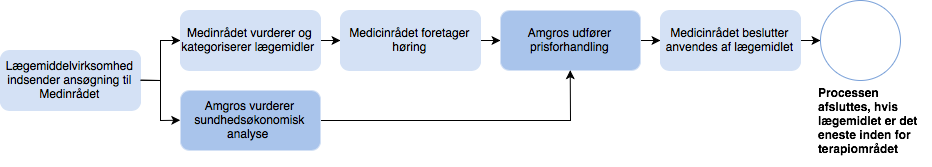
\includegraphics[width=1\textwidth]{billeder/Udbud.png} 
	\caption{Proces for vurdering af nye lægemidler.~\citep{DanskeRegioner2016}}
	\label{fig:Udbud}  
\end{figure}

Lægemiddelvirksomheder indsender som det første kliniske studier og sundhedsøkonomiske analyser til Medicinrådet med henblik på at ansøge om anvendelse af et nyt lægemiddel som standardbehandling~\citep{DanskeRegioner2016}. 

Efterfølgende kategoriserer Medicinrådet lægemidlet i merværdi på baggrund af ansøgningen samt en lægefaglig og statistisk vurdering.  Kategoriseringen inddeles i seks kategorier ud fra nuværende standardbehandling til stor, vigtig, lille, ingen, negativ og ikke-dokumenterbar merværdi~\citep{DanskeRegioner2016}. Yderligere høres Medicinrådets fagudvalg med henblik på at denne vurdering kan indgå i den samlede beslutning.~\citep{DanskeRegioner2016}

Parallelt med kategoriseringen forbereder Amgros en sundhedsøkonomisk analyse~\citep{DanskeRegioner2016} baseret på  samfundsomkostninger per patient for den nuværende og ansøgte behandling og samlede økonomiske konsekvenser for regionerne ved at anvende den ansøgende behandling ~\citep{Amgros2017, Amgros2017}. På baggrund af dette beregnes et prisinterval der danner grundlag for prisforhandlingen med lægemiddelvirksomhederne~\citep{DanskeRegioner2016}. 

Hvis den forhandlede pris er højere end den fastsatte kan lægemidlet ikke anbefales af Medicinrådet som standardbehandling~\citep{DanskeRegioner2016}. 
Er den forhandlede pris modsat lavere eller lig det fastsatte prisinterval og opfylder Medicinrådets faglige kriterier fremsendes en anbefaling til regionerne om anvendelse af lægemidlet som standardbehandling eller protokolleret anvendelse.
Ved protokolleret anvendelse tages lægemidlet i brug indtil der er tilstrækkeligt data til at Medicinrådet kan vurdere at lægemidlet kan anvendes som en fast behandling.~\citep{DanskeRegioner2016}

\section{Vurdering af ligeværdige lægemidler}
Hvis der er flere eksisterende lægemidler inden for samme terapiområde gennemgår lægemidlerne endnu en proces som fremgår af figur \ref{fig:Udbud1}. I denne proces har Medicinrådet til formål at udarbejde et national konsensus om anvendelse af lægemidlet inden for terapiområder~\citep{DanskeRegioner2016}. Processen varetages af fagudvalget, bestående af landets førende læger, der udarbejder forslag til fælles regionale behandlingsvejledninger. Disse forslag til behandlingsvejledningerne godkendes af Medicinrådet.~\citep{DanskeRegioner2016}

\begin{figure}[H]\centering
	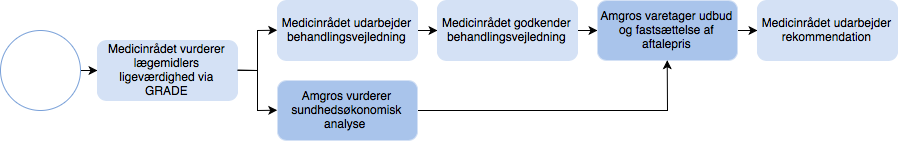
\includegraphics[width=1\textwidth]{billeder/Udbud1.png} 
	\caption{Proces for vurdering af ligeværdige lægemidler.~\citep{DanskeRegioner2016}}
	\label{fig:Udbud1}  
\end{figure}

Parallelt med udarbejdelse af forslag til behandlingsvejledning vurderer Amgros en sundhedsøkonomisk analyse~\citep{DanskeRegioner2016}. Amgros varetager herefter et udbud på baggrund godkendte  behandlingsvejledninger, hvorefter aftalepriser kan fastsættes og indføres i den sundhedsøkonomiske analyse.~\citep{DanskeRegioner2016}

Medicinrådet udarbejder til sidst en rekommandation, som omfatter det billigste lægemiddel, ud fra den behandlingsvejledningen fra fagudvalget og den sundhedsøkonomiske analyse~\citep{DanskeRegioner2016}. Rekommandationen indskrives herefter i behandlingsvejledningen og sendes til regionerne, der er ansvarlige for implementeringen af denne.~\citep{DanskeRegioner2016}
